\chapter{Implementation}
\chlab{implementation}


% Max. one figure at top of page
\setcounter{topnumber}{1}
\setcounter{bottomnumber}{1}
\setlength{\textfloatsep}{1em}
\renewcommand{\topfraction}{0.9}
\renewcommand{\bottomfraction}{0.9}
\renewcommand{\textfraction}{0.1}


A system for fragment-based molecule parameterisation has three distinct tasks: visualising a molecule, finding matching fragments for that molecule, and allowing for interaction with the molecule and its matching fragments. As these tasks can be performed in isolation, it has been decided to implement the molecule parameterisation tool as three separate systems.

The front-end of the system, where users will carry out the parameterisation process, will be called the Online tool for Fragment-based Molecule Parameterisation~(\oframp). This name will also be used to refer to the system as a whole, as it is the hart of the system and is dependent on the other systems. The molecule is also visualised in \oframp, but the - for this purpose essential - calculations of atom positions are done in the Online tool for Atom Position Calculations~(\oapoc). Finally, finding matching fragments and sorting them based on relevance is done by the Online tool for Molecule Fragment Finding~(\omfraf).

The complete network diagram for the fragment-based molecule parameterisation system is shown in \figref{network_diagram}. It is clear that \oframp{} is the central system, but that the more computation-intensive tasks are carried out by \oapoc{} and \omfraf{}. The remainder of this chapter will discuss each of the systems in more detail. Additionally, some more details can be found in \appref{implementation_extra}.


\begin{sidewaysfigure}[p]
\center
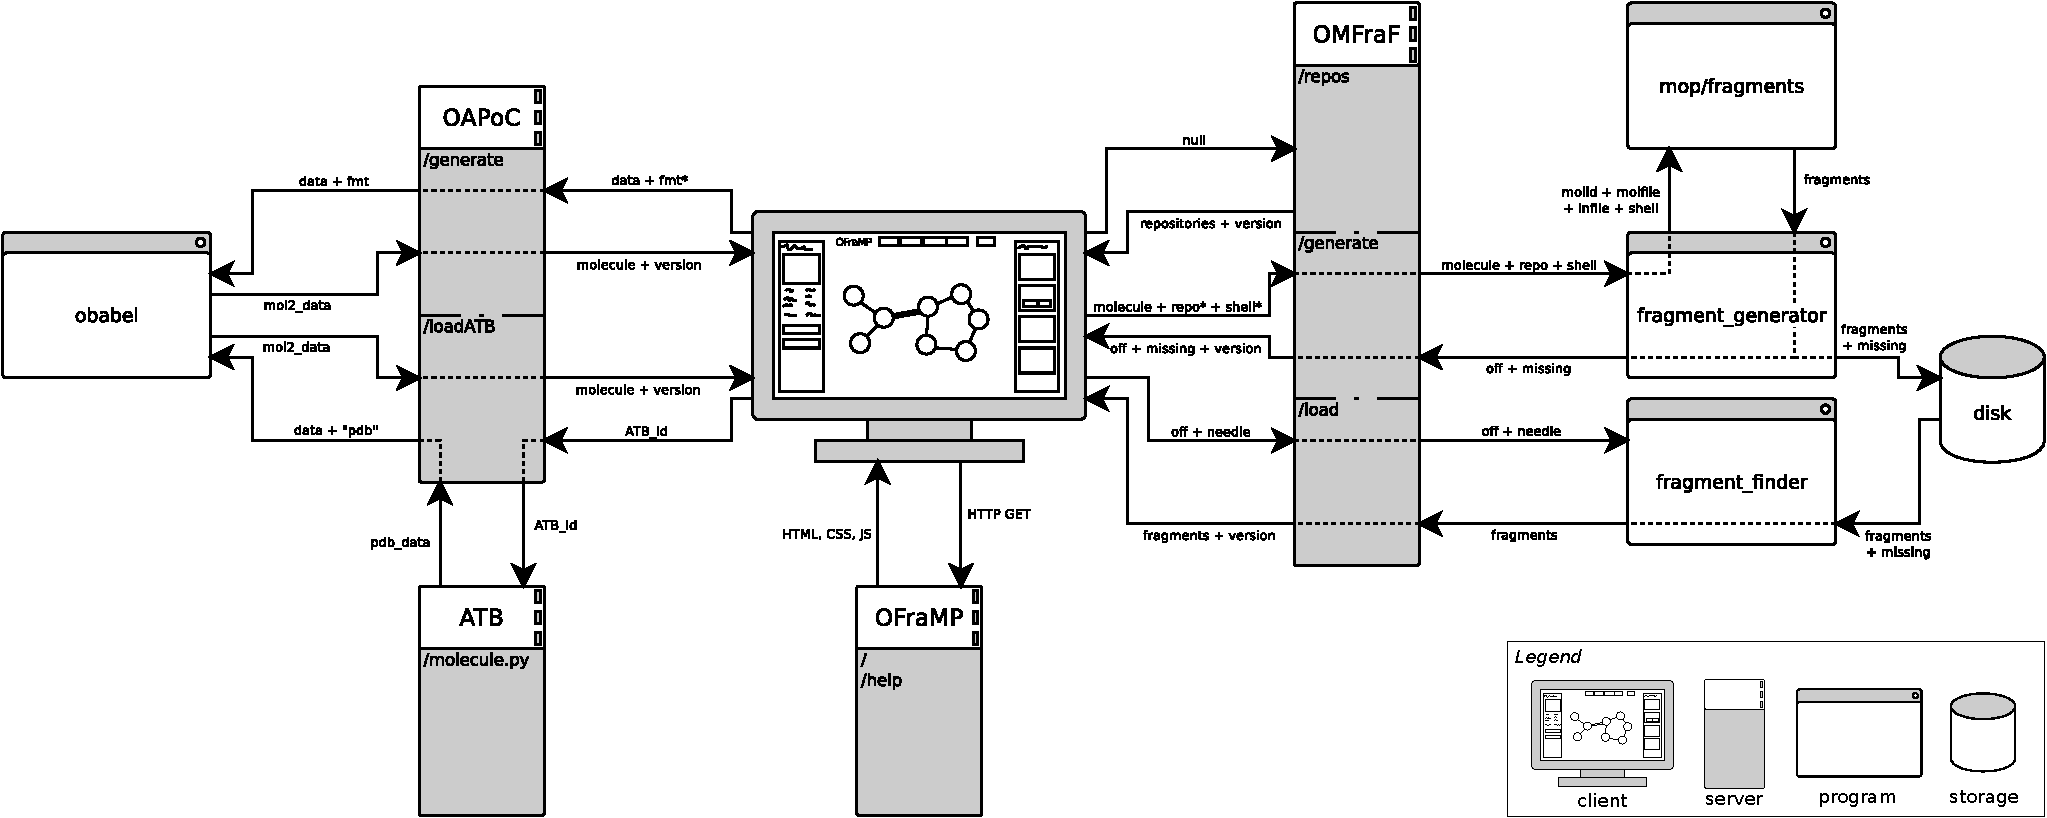
\includegraphics[width=\textwidth]{img/network_diagram.pdf}
\vspace{1em}
\caption{Network diagram of \oframp{} and its supporting systems.}
\figlab{network_diagram}
\end{sidewaysfigure}


\section[\oframp]{The Online tool for Fragment-based Molecule Parameterisation}
\oframp{} is the central part of the fragment-based molecule parameterisation system. It contains the user interface and connects with \oapoc{} and \omfraf{}. As discussed in \secref{platform}, it has been decided to implement the system as a web application. Following the current trend in web applications, \oframp{} has been implemented using the latest techniques from \verb|HTML5|, \verb|CSS3| and \verb|JavaScript|.

\subsection{Getting started}
\seclab{impl_starting}

Upon loading \oframp{} for the first time, one should see something similar to what is shown in \figref{impl_welcome}. It is explained what the tool is, and what it should be used for. Additionally, instructions are provided for first-time users and pointers are provided to the help pages. From this point, users can either start a short demonstration guide~(see \secref{impl_demo}) or submit a new molecule into the system~(see \secref{impl_inserting}).

\begin{figure}
\center
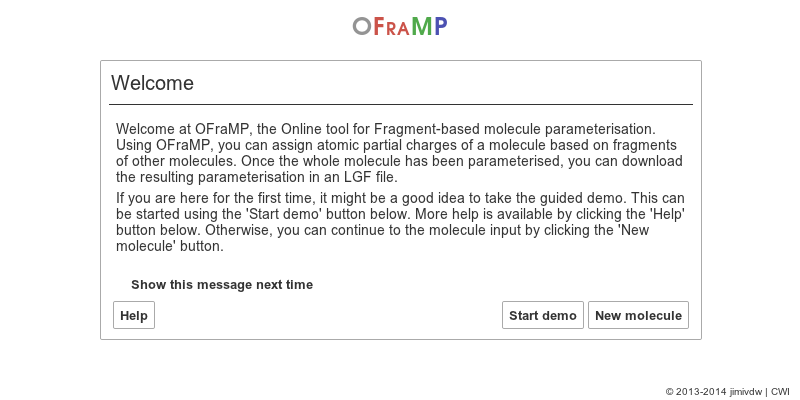
\includegraphics[width=.9\textwidth]{img/impl_welcome.png}
\caption{\oframp{} welcome screen.}
\figlab{impl_welcome}
\end{figure}

\Figref{impl_welcome} also shows the basic design of the system. It has been decided to go for a minimal look with a simple, purely textual logo. Besides the pastel colours of the logo, all text uses a dark shade of grey. Boxes and buttons all have a white background and a light grey, slightly rounded border.

Overly designed shiny elements are known to distract the user from his tasks~\cite{norman1990interfaces}~(see also \secref{design}). In some cases this may be beneficial, but for the purpose of finding a good molecule parameterisation this is undesirable. Therefore, this minimal design tries to make sure the user stays focused on the task that he needs to perform, rather than on using the tool. Furthermore, the tool still looks good and decent, which should prevent the users from distrusting it due to poor design~\cite{norman2002emotion}~(see also \secref{design}).

\subsubsection{Submitting a molecule}
\seclab{impl_inserting}

\begin{figure}
\center
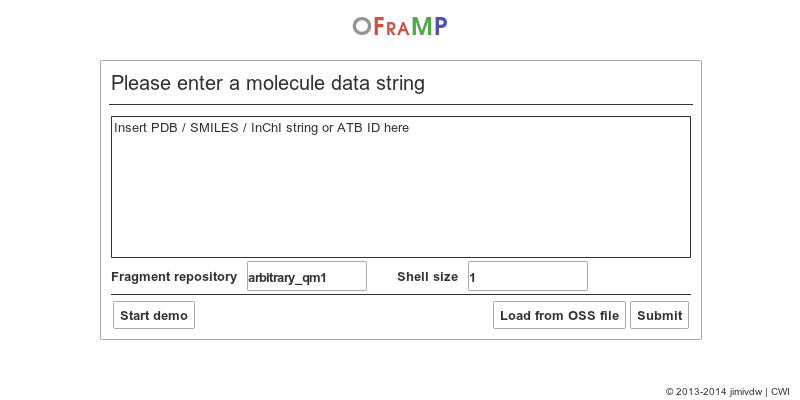
\includegraphics[width=.9\textwidth]{img/impl_inserting.png}
\caption{Insertion window for molecule data strings.}
\figlab{impl_inserting}
\end{figure}

In \figref{impl_inserting}, the insertion window for molecules is shown. This is where users should submit the molecules in a machine readable format, the so called molecule data string~(MDS). As discussed before, the system supports the \verb|PDB|, \verb|SMILES|, and \verb|InChI| formats, and the use of \verb|ATB ID|s~(see \secref{id_common}). When the MDS has been entered, the user can click the `Submit' button, after which the molecule will be displayed~(see \secref{impl_visualisation}).

Additionally, the user can adjust the fragment repository and shell size that are to be used for finding matching fragments of other molecules~(see \secref{impl_omfraf}). Furthermore, the demonstration mode~(see \secref{impl_demo}) can be started from this window as well, in case the user accidentally clicked the wrong button in the previous step. Finally, the user can load a so called \oframp{} State Storage~(OSS) file. These files can be created at any point in the parameterisation process and will store all progress up until that point. They can be loaded again at a later stage to continue the parameterisation process from that point.


\subsection{Visualisation}
\seclab{impl_visualisation}
% Once a molecule data string has been entered into the system, the positions of its atoms and the connections between them are retrieved from \oapoc~(see \secref{impl_oapoc}). This data is then transformed to a \verb|JavaScript| \verb|Molecule| instance, as can be seen in \figref{oframp_class}. \verb|Molecule| instances can be visualised using a \verb|MoleculeViewer|, which will draw the molecule onto an \verb|HTML| \verb|canvas|.

% \begin{figure}
% \center
% 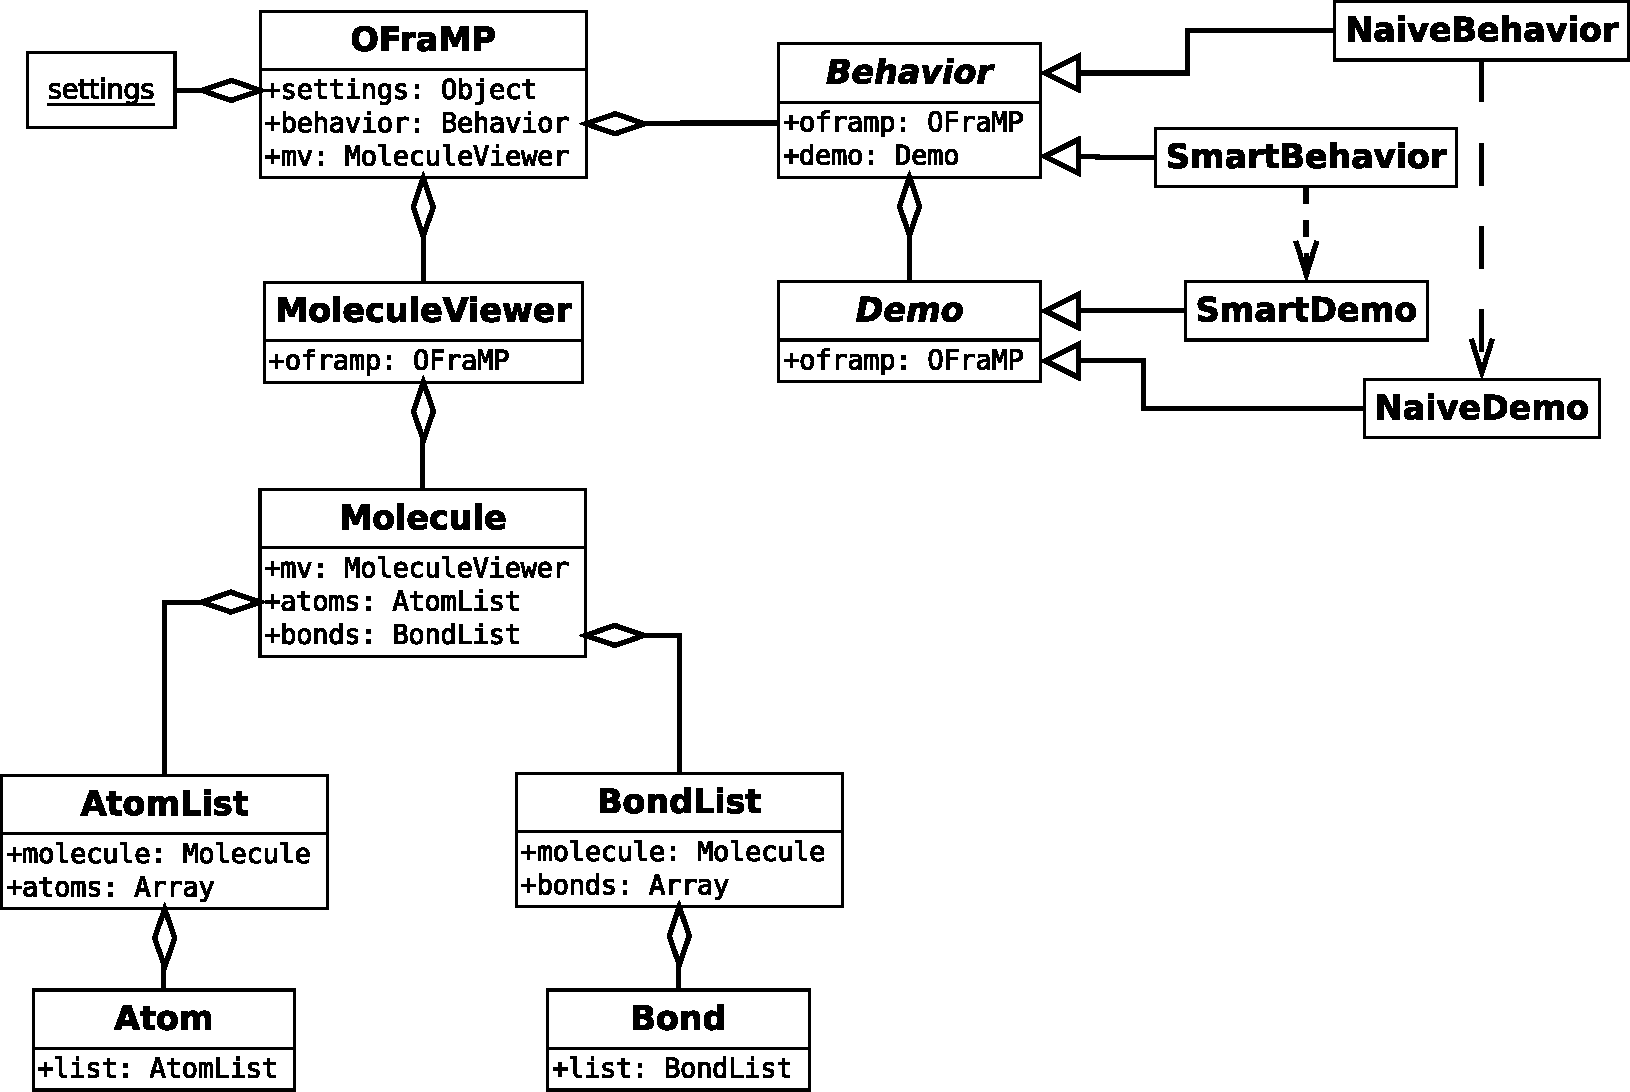
\includegraphics[width=\textwidth]{img/oframp_class.pdf}
% \caption{Simplified class diagram of \oframp.}
% \figlab{oframp_class}
% \end{figure}

Upon entering the \verb|SMILES| MDS `\verb|NCC(=O)CCO|' into \oframp, one should see something resembling what is shown in \figref{impl_visualising}. Similar to the molecule visualisation of the ATB~(see \figref{partial_charges} on \figpageref{partial_charges}), atoms are displayed as circles containing the atom type and with connecting lines that denote bonds. However, there are also a number of differences. First of all, charge group information is missing here, as these cannot be found before the atomic charges are available. Second, atom IDs (both on molecule and type scale) are left out. These are not considered to add any helpful information, and can therefore only be confusing. Third, obviously, the atom charges are missing, but they will also be added to the visualisation as soon as a matching fragment is selected~(see \secref{impl_parameterisation}). Fourth, as can be seen at the bottom-most $O$ atom, double bonds are visualised properly as a double line. The same is true for triple bonds~(triple line), and aromatic bonds~(dotted line on the inside of the aromatic cycle they are a part of).

\begin{figure}
\center
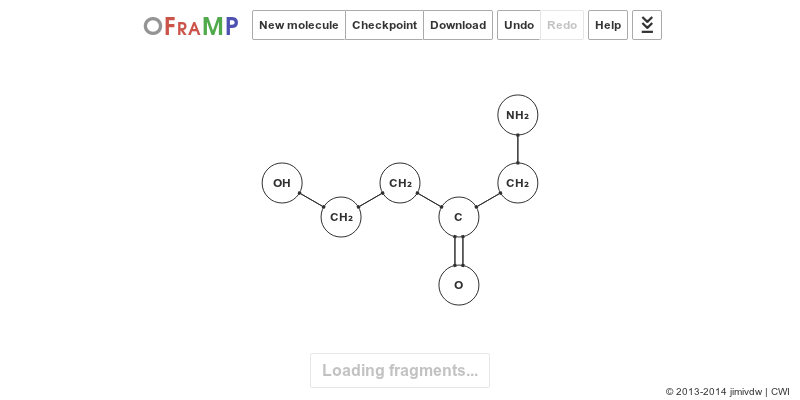
\includegraphics[width=.9\textwidth]{img/impl_visualising.png}
\caption{\oframp{} visualisation of \texttt{NCC(=O)CCO}.}
\figlab{impl_visualising}
\end{figure}

Finally, what is probably the most notable difference, is the fact that the $H$ atoms are grouped with their base atoms\footnote{This, along with many other settings, can be altered. See \secref{impl_settings} for more information.}. This means that they do not need to be drawn separately, leaving more space around the other atoms, thereby enhancing the overview of the complete molecule. Furthermore, in chemistry, it is quite common to have this combination. In many calculations, these groups can be treated as a single atom.

\subsubsection{Interaction}
At this point, the molecule can already be interacted with. It can be moved around by holding down the \emph{left} mouse button and dragging the mouse. This is mostly useful for larger molecules that may not completely fit on smaller screens. To provide further support for large molecules, the user has the opportunity to zoom in on certain sections of the molecule, or zoom out to make more atoms fit on the screen. Zooming can be done using the mouse wheel, or the zoom buttons located in the advanced controls settings, which can be opened using the button with the down pointing arrow~(see \figref{impl_visualising}).


\subsection{Parameterisation}
\seclab{impl_parameterisation}
As soon as the matching fragments for the molecule have been generated, the `Loading fragments...' message as visible in \figref{impl_visualising} will go away. It is now possible to start the fragment-based parameterisation process. The two implemented behaviours will be discussed in the next sections.

\subsubsection{Manual `naive' version}
In order to start the parameterisation process in the naive version of \oframp, a selection needs to be made. This selection can consist of a single atom or multiple \emph{connected} atoms, and should contain the atoms for which the user wants to find matching fragments. In order to make a single-atom selection, the user simply needs to click on that atom~(see \figref{select_1}). There are multiple ways to create multi-atom selections, the easiest of which is holding down the \emph{right} mouse button and dragging the mouse to create a selection rectangle as seen in \figref{select_2}. Alternatively, one could hold down the \verb|Ctrl| key while clicking atoms, or activate the selection modification mode, as seen in the selection details window in \figref{find_1}.

\begin{figure}
\centering
\begin{subfigure}[t]{0.45\textwidth}
\centering
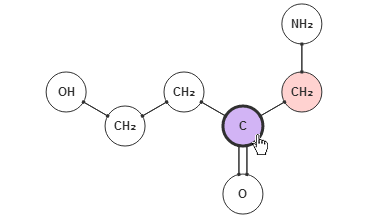
\includegraphics[width=\textwidth]{img/select_1.png}
\caption{Making a single-atom selection.}
\figlab{select_1}
\end{subfigure}%
\qquad
\begin{subfigure}[t]{0.45\textwidth}
\centering
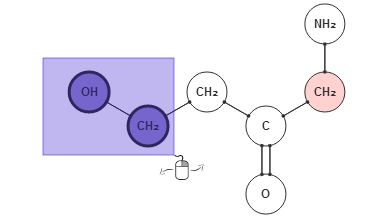
\includegraphics[width=\textwidth]{img/select_2.png}
\caption{Making a multi-atom selection.}
\figlab{select_2}
\end{subfigure}
\caption{\oframp{} atom selection.}
\figlab{selecting}
\end{figure}

When a selection has been made, matching fragments will automatically be retrieved from \omfraf~(see \secref{impl_omfraf}). These fragments will be shown in a sidebar on the right-hand side of the screen, and atom selection details will appear on the left-hand side~(see \figref{find_1}). Upon clicking a fragment, its charges will be previewed on the molecule~(see \figref{find_2}). The user then can decide if he wants to apply the charges of this fragment by clicking the `Select fragment' button that appears on the fragment, preview a different fragment by selecting another one, or inspect the fragment in the context of the molecule it originates from by clicking the `Show molecule' button.

\begin{figure}
\center
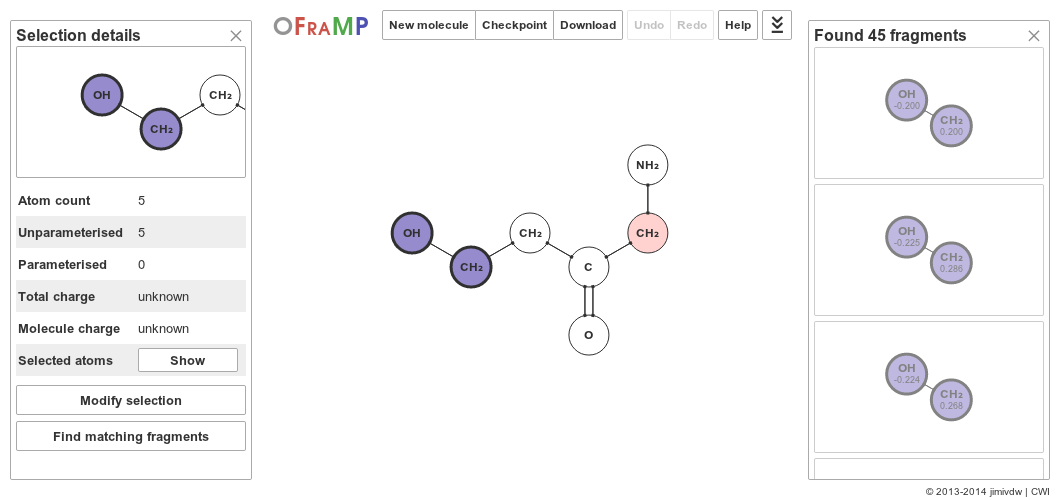
\includegraphics[width=.9\textwidth]{img/find_1.png}
\caption{Found fragments.}
\figlab{find_1}
\end{figure}

\begin{figure}
\center
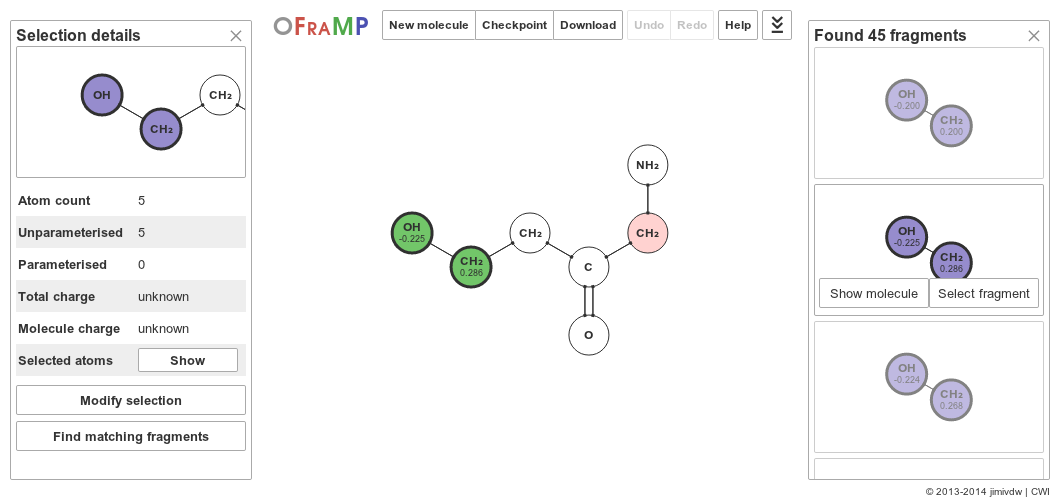
\includegraphics[width=.9\textwidth]{img/find_2.png}
\caption{Previewing the second found fragment.}
\figlab{find_2}
\end{figure}

As soon as the user clicks the `Select fragment' button, the charges from that fragment will be copied to the molecule. The selection will be cleared, and, because of that, the list of found fragments will be closed. The user can now select another atom or set of atoms he wants to parameterise, in order to complete the parameterisation. This will be discussed in more detail in \secref{impl_completing}.


\subsubsection{Semi-automatic `smart' version}
In the smart version of \oframp, the parameterisation process can be started by clicking the `Start parameterising' button shown in \figref{find_3}. The system will now automatically select a random atom \emph{at the edge of the molecule} for which fragments will be retrieved. The molecule will be centred on that molecule, and the charges of the best found fragment will be previewed~(see \figref{find_4}). In that figure, the atoms with the green background and the thicker border are the atoms occurring in the found fragment.

\begin{figure}
\center
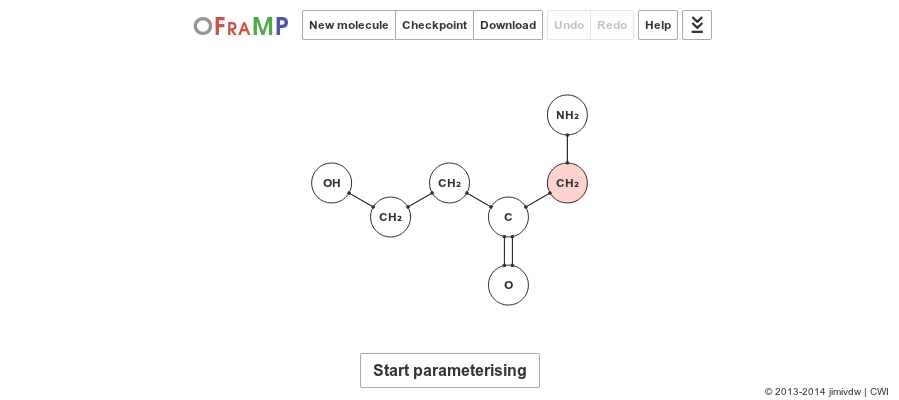
\includegraphics[width=.9\textwidth]{img/find_3.png}
\caption{Ready to start parameterisation.}
\figlab{find_3}
\end{figure}

\begin{figure}
\center
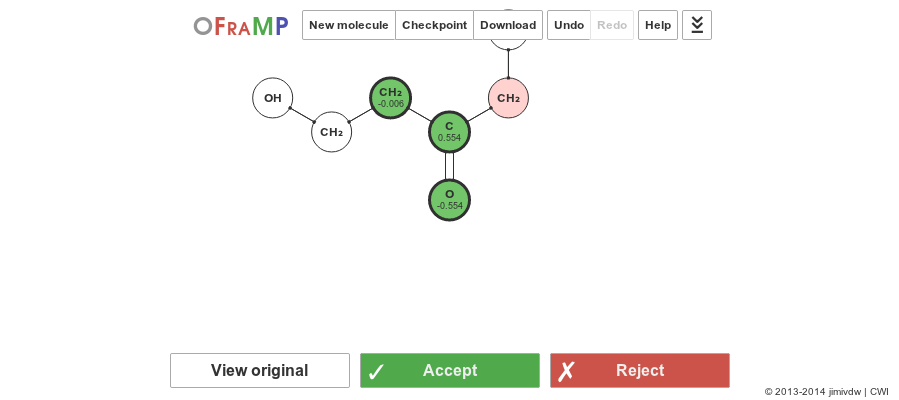
\includegraphics[width=.9\textwidth]{img/find_4.png}
\caption{Previewing a found fragment.}
\figlab{find_4}
\end{figure}

The user now needs to decide whether he thinks this proposed fragment is a good match with the molecule. In order to help him to make this decision, he can view the fragment in the context of the molecule it originates from by clicking the `View original' button~(see \figref{find_4}). When he rejects the fragment, the next best fragment will be previewed, up until the point where there are no found fragments left. Either the final fragment needs to be accepted then, or the user can undo some of his rejections using the `Undo' button at the top of the page.

Upon acceptance of a fragment, the charges of that fragment are copied to the molecule. The system will then find another \emph{unparameterised} atom for which fragments will be proposed. This atom is preferably connected to the last accepted fragment, or, when no unparameterised atoms are neighbouring that fragment, positioned on the edge of the molecule. The user can now continue to parameterise the molecule, which will be discussed in more detail in \secref{impl_completing}.


\subsection{Completing parameterisation}
\seclab{impl_completing}
Upon continuing to parameterise a molecule, it is possible to encounter fragments that contain atoms to which a charge has already been assigned. The atoms in question are given a yellow background, as can be seen in \figref{conflict}. When such fragment is selected, it is dependent on which \oframp{} version is used what will happen. As discussed in \secref{id_smart}, the smart version will automatically assign the average of the two charges. In the naive version of the tool, a pop-up will be shown, asking the user to pick a solution method for solving the charge conflict.

\begin{figure}
\center
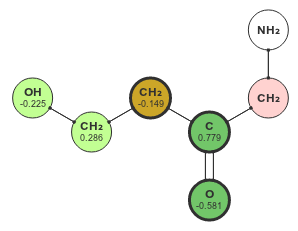
\includegraphics[height=140px]{img/conflict.png}
\caption{Molecule with a charge conflict.}
\figlab{conflict}
\end{figure}

In some cases, it can happen that no matching fragments are found for an atom. This will be indicated by colouring that atom with a pink/red background, as can be seen for the rightmost $CH_{2}$ group in \figref{conflict}~(and also figures \ref{figure:selecting}, \ref{figure:find_1}, \ref{figure:find_2}, \ref{figure:find_3}, and \ref{figure:find_4}). Upon selecting these atoms, no fragments will be returned. It is still possible to parameterise them manually, in the same way one can fine-tune atom charges~(see below).

When a charge has been assigned to all \emph{parameterisable} atoms~(i.e. atoms for which fragments can be found), the user will be notified of this with a pop-up similar to the one shown in \figref{finished}. As it says there, he can now fine-tune the atom charges~(see below), download the resulting parameterisation, or enter a new molecule.

\begin{figure}
\center
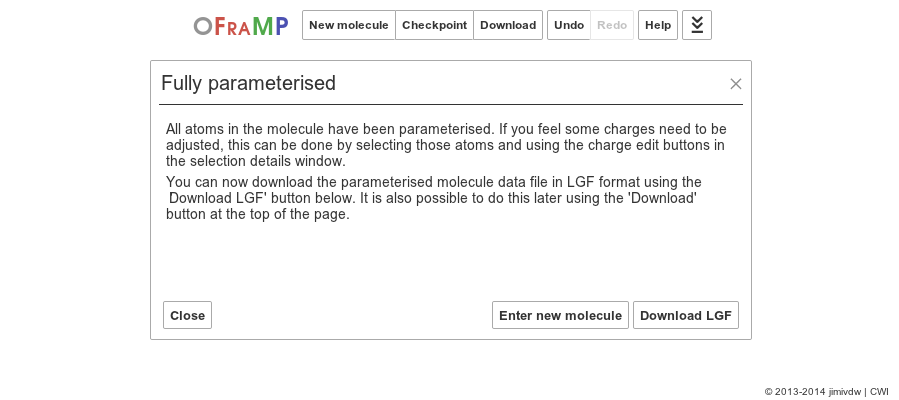
\includegraphics[width=.9\textwidth]{img/finished.png}
\caption{Notification of parameterisation completion.}
\figlab{finished}
\end{figure}


\subsubsection{Fine-tuning charges}
\seclab{impl_finetuning}
Charges of fragments of molecules will often not precisely match with the charges of another molecule. Therefore, the user has the ability to manually adjust atom charges when he wishes to do so. In order to do this, he needs to select the atoms he wishes to adjust the charges for. In the selection details panel, the `Show' button in the `Selected atoms' row should be clicked. A table containing detailed information about the atom will be shown, as can be seen in \figref{editing}.

\begin{figure}
\center
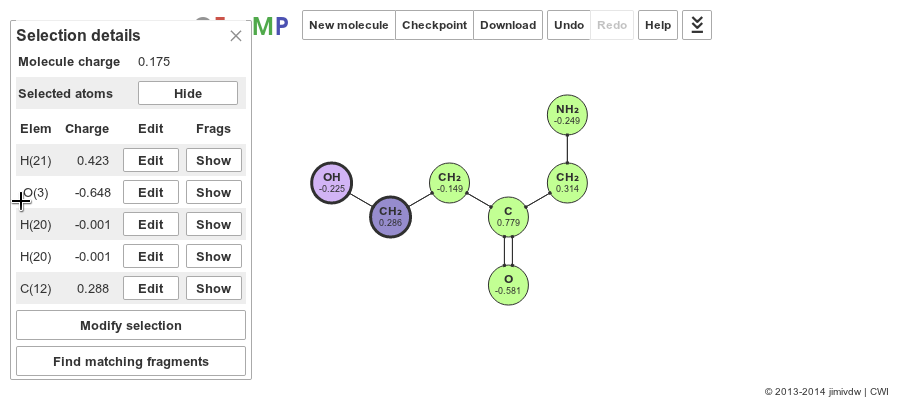
\includegraphics[width=.9\textwidth]{img/editing.png}
\caption{Manually fine-tuning or adding charges.}
\figlab{editing}
\end{figure}

The atom details table contains information about all atoms that are part of the selection. Hovering with the mouse over a row will highlight the corresponding atom in the molecule, which can be seen for the $O$ atom in \figref{editing}. The `Elem' column contains the atom element and its \verb|IACM atom type|~(in parentheses). The charge is shown, which can be edited by clicking the `Edit' button in the column next to it. Finally, clicking the `Show' button in the `Frags' column, will show the fragments that were used to get the current atom charge, as discussed in \secref{id_common}.


% \subsubsection{Downloading results}
% \seclab{impl_downloading}
% When the user feels he is completely done, he can download the resulting parameterisation of the molecule by clicking the `Download' button at the top of the page. This will give him the result in the \verb|LEMON Graph File|~(LGF) format~\cite{dezso2011lemon}. This format has been chosen as it is used by, among others, the fragment finding system~(see \secref{mop_fragments}), and because it is a flexible format that can easily be generated. This file will contain all atoms' element types, \verb|IACM| and charge, and all bonds between the atoms. It can currently not be imported back into the system, but support for that may be added at a later stage.


\subsection{Other features}
Besides the features required for the normal use of \oframp{} described in the previous sections, some other features have been developed to further improve the user experience. The following sections will discuss the Demo mode~(\secref{impl_demo}), modification of visualisation parameters~(\secref{impl_settings}), and the \oframp{} Help pages~(\secref{impl_help}).

\subsubsection{Demo mode}
\seclab{impl_demo}

In order to help new users learn to use the system, a Demo mode has been implemented. Both implementations of \oframp{} have their own Demo implementation, suited for that version. It can be started by clicking the `Start demo' button, as discussed in \secref{impl_starting}.

\begin{figure}
\center
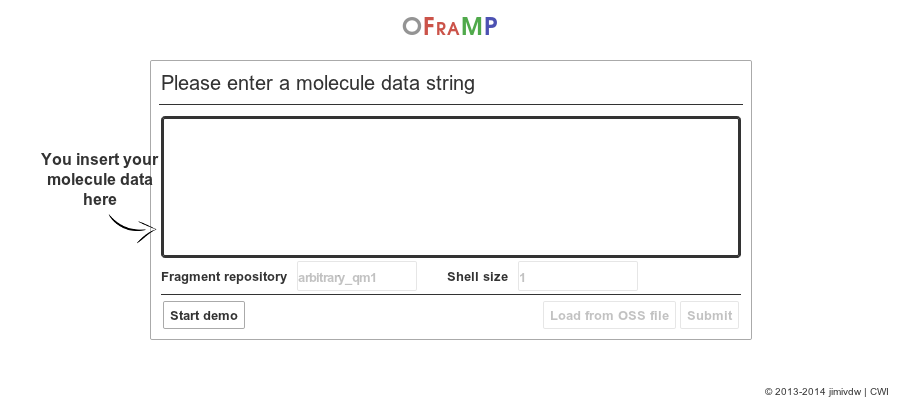
\includegraphics[width=.9\textwidth]{img/demo_1.png}
\caption{Start of both Demo modes.}
\figlab{demo_1}
\end{figure}

The Demo mode will guide the user through the basic steps that are required to completely parameterise a molecule. He will receive detailed instructions on what buttons to press at which time, and other buttons will be disabled. Upon starting the demo mode, one should see something similar to what is shown in \figref{demo_1}. A simple molecule data string will be automatically be entered into the input field, to ensure that the system can easily be explained with that molecule.

\begin{figure}
\center
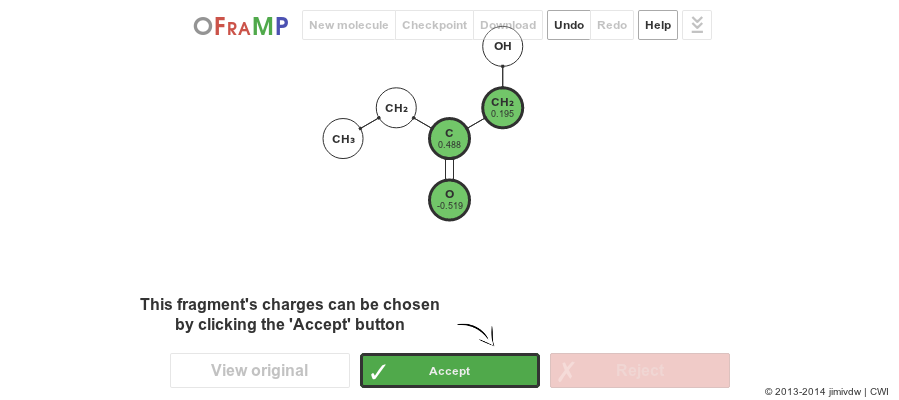
\includegraphics[width=.9\textwidth]{img/demo_2.png}
\caption{Parameterisation in the Demo mode of \oframp{} smart.}
\figlab{demo_2}
\end{figure}

The user will be guided through most aspects of \oframp, including interaction with the molecule visualisation, fragment selection and comparison~(see \figref{demo_2}), and retrieving the results. By allowing for user interaction with the demonstration, it is hoped that the Demo mode will not only serve as an example, but also help the user to learn how to use \oframp{} in a different case. This way, it should have both the benefits of learning by example and learning by familiarisation~\cite{sweller1994cognitive}~(see also \secref{id_learning}).

\subsubsection{Modifying visualisation parameters}
\seclab{impl_settings}
Research on both data visualisation in general~\cite{gallopoulos1994computer}~(see also \secref{design}) and molecule visualisation in particular~\cite{aksela2008computer,taylor2013interface}~(see also \secref{ms_requirements}) has shown that being able to modify visualisation parameters at runtime will greatly enhance the user experience and help him to carry out the task he intends to complete. Therefore, most of the molecule visualisation parameters, such as the atom radius or grouping of $H$ atoms, can dynamically be modified. % It has been implemented using a slight modification of the \verb|JavaScript| library \verb|dat-gui|~\cite{data2011dat}.
This is not included in the demo, but information about it can be found on the \oframp{} Help pages.

\subsubsection{Help}
\seclab{impl_help}

\begin{figure}
\center
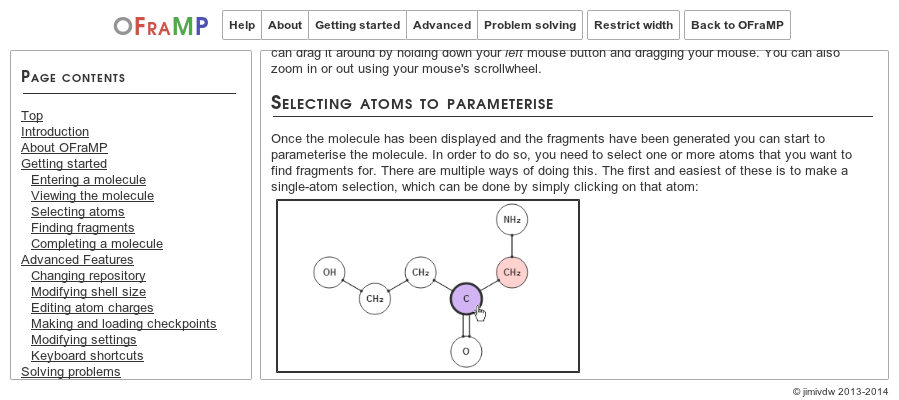
\includegraphics[width=.9\textwidth]{img/help.png}
\caption{\oframp{} Help for the naive version: selection instructions.}
\figlab{help}
\end{figure}

Despite the fact that using \oframp{} should be intuitive, and the presence of its Demo mode, some users prefer textual instructions. Furthermore, some of the advanced features that are not covered by the demonstration need to be documented as well. Therefore, a Help page has been created~(see \figref{help}). It includes a little introduction on \oframp, basic instructions on how to parameterise a molecule, detailed descriptions of the advanced features, and instructions on how to solve common problems.

As can be seen in \figref{help}, the Help page uses the same type of design as \oframp, consisting of white boxes with grey, slightly rounded borders. Once again, this simplicity makes sure users are not distracted by the interface, but will be able to find the information they need. Furthermore, the consistency in the layout follows the interaction design principles~\cite{norman2010gestural,blair2008user}~(see also \secref{id_principles}), to enhance user satisfaction.


\section[\oapoc]{The Online tool for Atom Position Calculations}
\seclab{impl_oapoc}

The atom positions and bonds that are required for visualising molecules are found by \oapoc, which has been implemented using the \verb|Python| web framework \verb|Django|. As can be seen in \figref{network_diagram} on \figpageref{network_diagram}, \oapoc{} can calculate the molecule data either from an \verb|ATB ID|, or a molecule data string in an optionally specified format\footnote{When not provided, the format will be guessed automatically, which may be error-prone.}. Internally, this input will be converted to some other format that includes the atom position and bond information, and can easily be parsed and interpreted.

For making this conversion, it has been decided to go with \verb|Open Babel|~\cite{oboyle2011open}~(see also \secref{ms_visualisation}). This tool can be used easily and for free, and has support for most common MDS formats.

% The data that \verb|obabel| returns will be parsed and converted to a \verb|JSON| object, such that it can be sent to the client running \oframp. Additionally, \verb|IACM| atom types are calculated, following the algorithm presented by Malde~et.~al.~\cite{malde2011automated}. These atom types are needed later to find matching fragments for the molecule.

% \subsection{From ATB}
% When an \verb|ATB ID| is supplied to \oapoc, the molecule data string will be retrieved from the ATB. For all its molecules, the ATB stores a \verb|PDB| file, which is one of the formats that \oapoc{} supports. This file will be downloaded, and its contents will be used as the MDS for finding the molecule data.

% \subsection{Open Babel}
% \seclab{oapoc_obabel}
% For converting molecule data strings from one format to another, it has been decided to go with \verb|Open Babel|~\cite{oboyle2011open}. This tool can be used easily and for free, and has support for most common MDS formats. 

% Needs to be merged properly still!
For this purpose, the choice has been made to use the \verb|Python| web framework \verb|Django| for that part. This framework can easily be set up on various platforms and provides a wide span of features.Additionally, it performs quite well, and is known to provide good atom positions.

% From \oapoc, the \verb|Open Babel| executable \verb|obabel| takes an MDS and the format that MDS uses. \verb|obabel| will then convert the MDS to the \verb|Mol2| format. This format has been chosen as it can easily be parsed and contains information on atom positions and bonds. Furthermore, it does not leave out the \verb|H| atoms, which some other formats do. For some applications this is fine, but for \oframp{} it is required to have all \verb|H| atoms.


\section[\omfraf]{The Online tool for Molecule Fragment Finding}
\seclab{impl_omfraf}
Perhaps the most important part of the fragment-based molecule parameterisation system is the part that finds matching fragments for the input molecule. In the current implementation, this is done by \omfraf. Provided with the input molecule, a repository of molecules that can be queried for fragments, and a shell size within which the atoms should match, the tool can generate a list of matching fragments. As some complex chemical concepts need to be understood to determine whether a similar fragment is a good match, an external tool needs to be used for this. In \omfraf, fragments are generated using El-Kebir's \verb|fragments| tool, from the \verb|mop| project~\cite{elkebir2014molecule}.

% \subsection{Getting the repositories}
% In order to be able to select a repository, the user needs to know what repositories are available. As can be seen in \figref{network_diagram}, a list of repositories can be retrieved by sending an empty \verb|JSON| object to \omfraf's \verb|/repos| URL. As of now, this list consists of only the repository titles. Later, this may be extended to also include the list of molecules that are contained in that repository, combined with functionality to exclude individual molecules. This will be discussed in more detail in \secref{futwork}.

% \subsection{Generating fragments}
% \seclab{impl_generating}
% Before any fragments can be found, all matching fragments for the molecule need to be generated. As some complex chemical concepts need to be understood to determine whether a similar fragment is a good match, an external tool needs to be used for this. In \omfraf, fragments are generated using El-Kebir's \verb|fragments| tool, from the \verb|mop| project~\cite{elkebir2014molecule}.

% As can be seen in \figref{network_diagram}, the \verb|fragments| tool has been wrapped in a program called \verb|fragment_generator|. For every molecule in the provided repository, this tool will retrieve the matching fragments with the input molecule, transform them into a slightly more manageable format, combine the fragments of all molecules, and store them to disk in the so-called \omfraf{} Fragments File~(OFF) format. The name of this file will be sent back to the \oframp{} user, such that he can query for fragments later. Along with the fragment file's name, a list of atoms for which no matching fragments could be found is sent to the user, which will allow for indicating these atoms in the molecule visualisation~(see \secref{impl_completing}).

% \subsubsection{mop/fragments}
Provided with a target molecule file and another input molecule file, the \verb|fragments| tool will find all maximal fragments in the input molecule file that match with parts of the target molecule. It will score the fragments based on, among others, their size, such that they can be presented in order of relevance. In order to be a match, not only the atoms that are part of the fragment must match; the atoms in a so-called shell around the fragment should also match.

\begin{figure}
\centering
\begin{subfigure}[t]{0.29\textwidth}
\centering
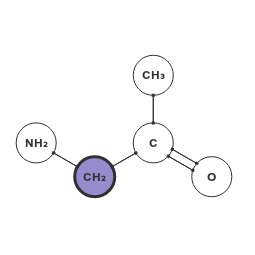
\includegraphics[width=\textwidth]{img/shell_1.png}
\caption{Target atoms that should occur in any fragment, highlighted in blue.}
\figlab{shell_1}
\end{subfigure}%
\qquad
\begin{subfigure}[t]{0.29\textwidth}
\centering
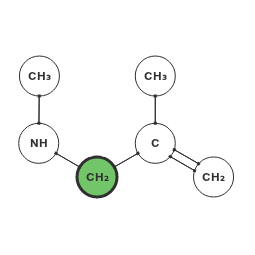
\includegraphics[width=\textwidth]{img/shell_2.png}
\caption{Matching fragment, highlighted in green.}
\figlab{shell_2}
\end{subfigure}%
\qquad
\begin{subfigure}[t]{0.29\textwidth}
\centering
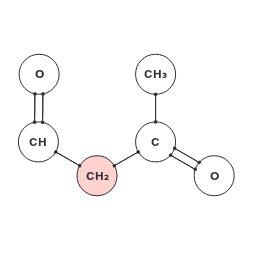
\includegraphics[width=\textwidth]{img/shell_3.png}
\caption{Non-matching fragment, highlighted in red / pink.}
\figlab{shell_3}
\end{subfigure}
\caption{Fragment matching with shell size $1$.}
\figlab{shell_matching}
\end{figure}

\Figref{shell_matching} shows the concepts of fragment matching for a shell size of $1$. As we can see, in \figref{shell_2}, the neighbouring atoms of the selected $CH_{2}$ group are $C$ and $N$ atoms, just like in \figref{shell_1}. In \figref{shell_3}, the $C$ atom to the right still matches, but the atom on the left-hand side no longer matches, as this is a $C$ atom. Would the shell size be increased further, to $2$, for example, then the second fragment would no longer be matching, due to the $CH_{3}$ group connected to the $NH$ group, and the $CH_{2}$ group connected to the $C$ atom to the right. The former is not present in the original molecule at all, the latter should be an $O$ atom to match.

% \subsection{Finding fragments}
% \seclab{impl_finding}
% Once the fragments have been generated, the user of \oframp{} will be able to start finding fragments. The selected atom(s) and OFF filename will be sent to \omfraf, which will invoke the \verb|fragment_finder|. This program will load the fragments from the OFF file, and select those in which \emph{all} selected atoms are present. Those fragments will be ordered based on the score that was assigned to them by the \verb|fragments| tool, and are returned to the \oframp{} front-end such that they can be used in the parameterisation process.

Once the fragments have been generated, the user of \oframp{} will be able to start finding fragments. For this purpose, the generated list of fragments will be queried to retrieve the fragments in which a certain atom or set of atoms~(the selection) occurs.
